贝\documentclass[UTF8]{ctexart}
\usepackage{geometry, CJKutf8}
\geometry{margin=1.5cm, vmargin={0pt,1cm}}
\setlength{\topmargin}{-1cm}
\setlength{\paperheight}{29.7cm}
\setlength{\textheight}{25.3cm}

% useful packages.
\usepackage{amsfonts}
\usepackage{amsmath}
\usepackage{amssymb}
\usepackage{amsthm}
\usepackage{enumerate}
\usepackage{graphicx}
\usepackage{multicol}
\usepackage{fancyhdr}
\usepackage{layout}
\usepackage{listings}
\usepackage{float, caption}

\lstset{
    basicstyle=\ttfamily, basewidth=0.5em
}

% some common command
\newcommand{\dif}{\mathrm{d}}
\newcommand{\avg}[1]{\left\angle #1 \right\angle}
\newcommand{\difFrac}[2]{\frac{\dif #1}{\dif #2}}
\newcommand{\pdfFrac}[2]{\frac{\partial #1}{#2}}
\newcommand{\OFL}{\mathrm{OFL}}
\newcommand{\UFL}{\mathrm{UFL}}
\newcommand{\fl}{\mathrm{fl}}
\newcommand{\op}{\odot}
\newcommand{\Eabs}{E_{\mathrm{abs}}}
\newcommand{\Erel}{E_{\mathrm{rel}}}

\begin{document}

\pagestyle{fancy}
\fancyhead{}
\lhead{张广, 3230105121}
\chead{数据结构与算法第四次作业}
\rhead{Oct.16th, 2024}

\section{测试程序的设计思路}

首先,我创建了一个 List<int> 对象 lst,然后使用了 \verb|push_back| 和 \verb|push_front| 方法分别向链表的尾部和头部插入数据。接下来,我测试了 \verb|pop_back| 和 \verb|pop_front|,验证链表的元素删除操作。通过使用迭代器,我测试了链表的前向遍历和后向遍历,确保迭代器的 ++ 和 \verb|--| 操作符都能正常工作。

此外,我测试了 insert() 和 erase(),分别在链表中插入和删除元素。我也特别测试了 erase(iterator from, iterator to) 来验证删除范围内多个元素的功能。最后,我使用了 clear() 方法清空链表,并测试了链表在被清空后是否正确返回大小和是否为空。

为了全面覆盖 List 类的功能,我还测试了拷贝构造函数、移动构造函数、拷贝赋值运算符和移动赋值运算符,确保对象在各种操作下能正确复制或移动。

\section{测试的结果}

所有测试均成功通过。程序能够正确地插入、删除、遍历和修改链表中的元素。在迭代器操作中,前向和后向遍历都能正常工作,且删除操作没有引发迭代器失效的问题。范围删除功能 erase(iterator from, iterator to) 也正确地删除了指定范围内的元素。

我使用 valgrind 工具对程序进行了内存泄漏的检测,结果显示程序不存在任何内存泄漏问题,所有动态分配的内存都得到了正确的释放。

测试结果的详细输出如下:
\begin{verbatim}
Forward traversal: 0 1 2 3 4 
Backward traversal: 4 3 2 1 0 
After push_front: 2024
After pop_back: 2024 0 1 2 3 
After pop_front: 0
List size: 4
List is empty: false
After insert: 0 2024 1 2 3 
After erase: 0 2024 1 2 
After clear, list size: 0
List is empty after clear: true
List3 (copy of list2): 10 20 30 
List4 (moved from list2): 10 20 30 
List6 after move assignment: 10 20 30 
List7 after range erase: 4 5 
List8 after copy assignment: 10 20 30 
\end{verbatim}

使用valgrind检测无内存泄漏的截图如下:
\begin{figure}[H]
    \centering
    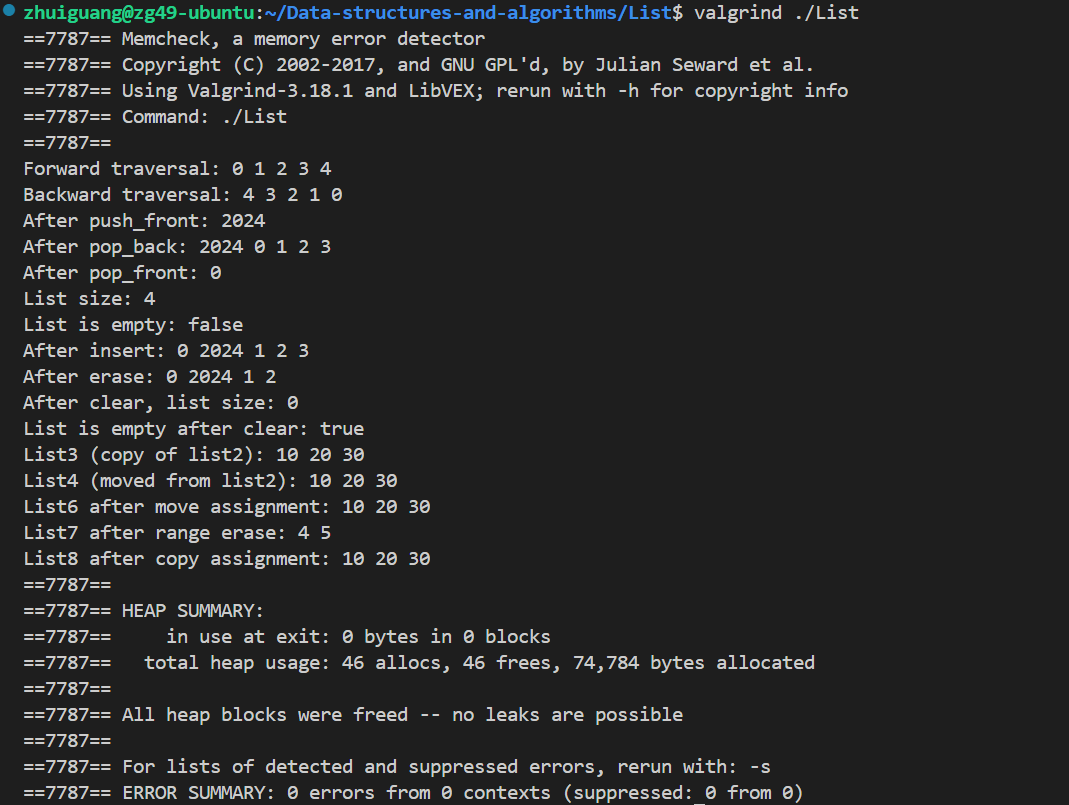
\includegraphics[width=1\linewidth]{内存无泄漏.png}
    \caption{无内存泄漏}
    \label{fig:enter-label}
\end{figure}

\section{总结}

在List.cpp中我验证了 List 类中的所有功能,包括插入、删除、遍历、拷贝和移动等操作。所有测试均表明 List 类工作正常,并且通过valgrind确保了该程序无内存泄漏

\end{document}


%%% Local Variables: 
%%% mode: latex
%%% TeX-master: t
%%% End: 
